\section{Methodology}
\label{sec:method}

\subsection{Problem Formulation}

Let $\mathcal{D} = \{(x_i, y_i)\}_{i=1}^{N}$ denote the transaction log, where
$x_i \in \mathbb{R}^{35}$ is the feature vector of transaction $i$ and
$y_i \in \{0,1\}$ indicates fraud. We learn a scoring function
$f_\theta : \mathbb{R}^{35} \to [0,1]$ and a threshold $\tau$ such that
\[
    \hat{y}_i = \mathbb{1}\left[f_\theta(x_i) \geq \tau\right].
\]
The threshold $\tau$ is not learned jointly with $\theta$; it is selected to
satisfy a business constraint on precision, as detailed in
Section~\ref{sec:leakage}.

\subsection{Pipeline Architecture}

\begin{figure}[h!]
\centering
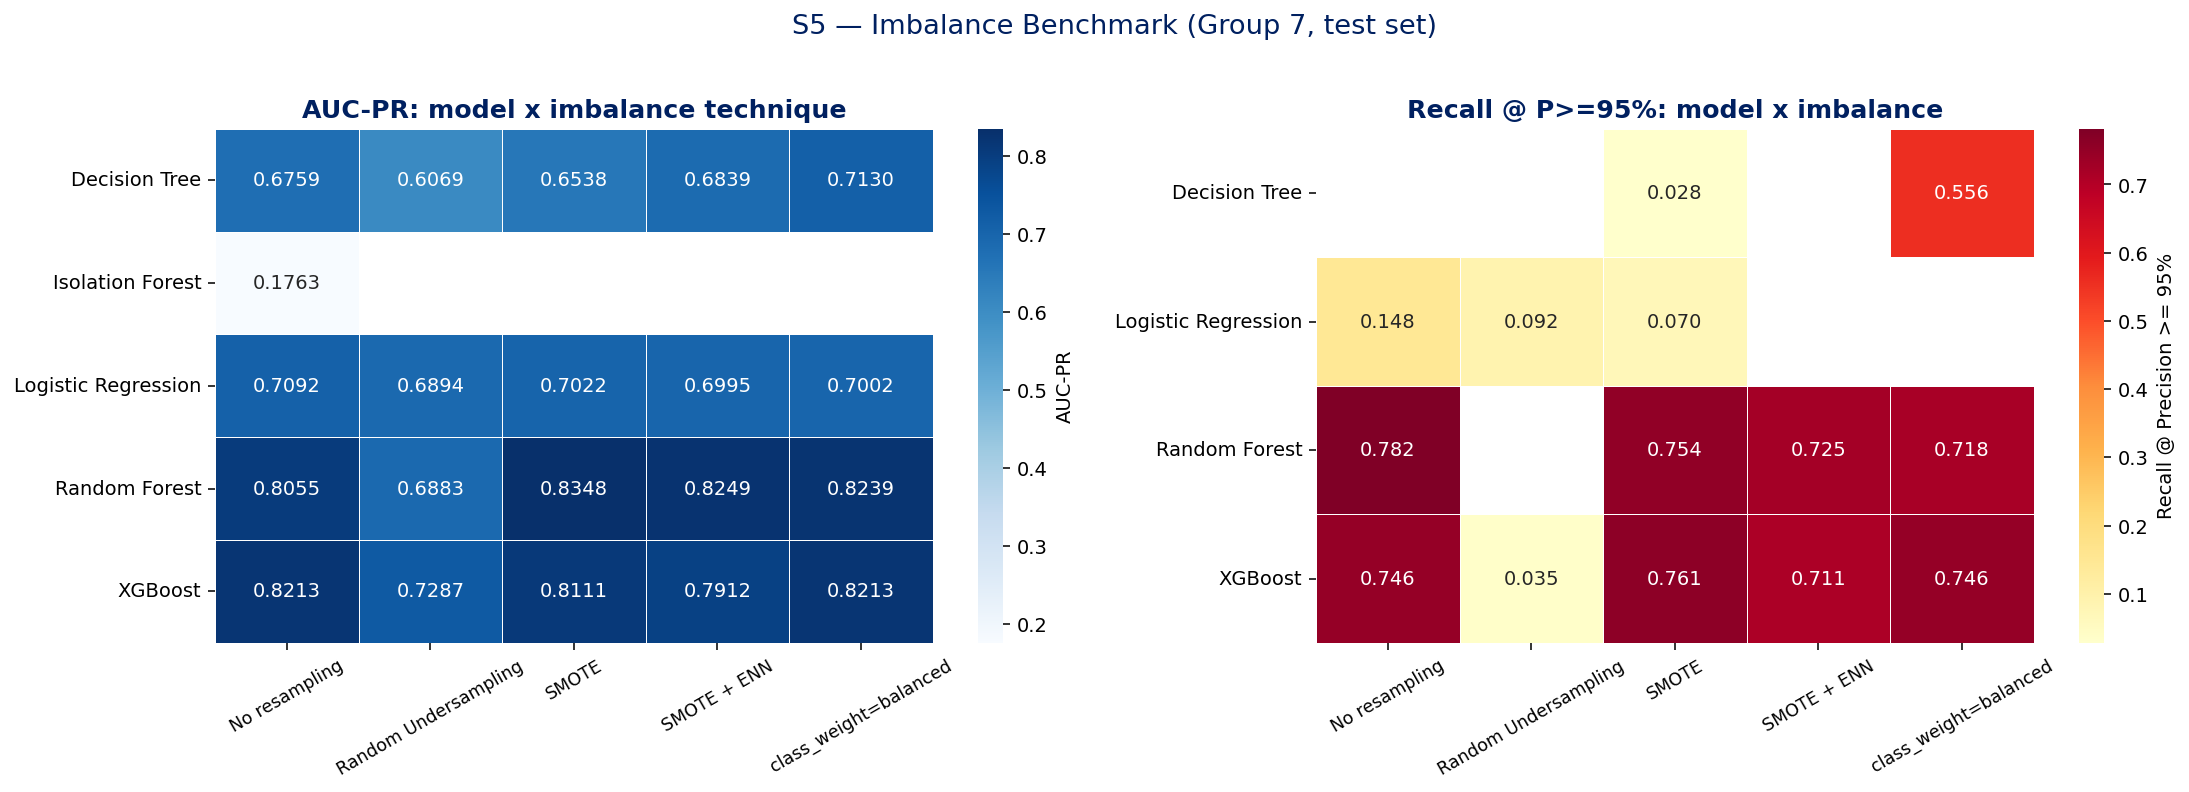
\includegraphics[width=0.90\textwidth]{Images/charts/s5_heatmap_model_x_imbalance.png}
\caption{Heatmap of Average Precision across the five model families and
five imbalance techniques. Of the 25 cells, 21 were executed: Isolation
Forest was run only without resampling, since it has no class label to
resample. The highest Average Precision in the grid (0.8348) is attained by
Random Forest combined with SMOTE at the \emph{1:10} ratio --- the mildest
oversampling that still changes the class prior. The configuration we finally selected, Random Forest with SMOTE at
1:100, attains 0.8239: it trades 0.011 Average Precision for a markedly more
stable ranking and a higher recall at the precision-constrained operating
point. Random Undersampling degrades every model family.}
\label{fig:heatmap}
\end{figure}

The pipeline has six stages, executed as six reproducible Jupyter notebooks
(\texttt{00}--\texttt{05}) under a single random seed.

\paragraph*{Stage 1 --- Data acquisition and quality control.}
The raw dataset contains 284{,}807 rows and 31 columns. We removed 1{,}081
exact duplicate rows (1{,}062 legitimate, 19 fraudulent), leaving 283{,}726
transactions with 473 frauds. No missing values were present, and no amount was
negative. We deliberately \emph{retained} outliers: extreme amounts are
genuinely informative signals of fraud, and removing them would bias the
detection task.

\paragraph*{Stage 2 --- Reproducible stratified split.}
A single stratified 70/30 split (seed 42) yields 198{,}608 training rows with
331 frauds and 85{,}118 test rows with 142 frauds. The split is serialised
once to \texttt{split\_with\_features.joblib} and re-loaded by every downstream
notebook, so no experiment can accidentally observe a different partition.

\paragraph*{Stage 3 --- Feature engineering.}
Five features were derived from \texttt{Time} and \texttt{Amount}:
\texttt{Hour\_of\_Day} $= (\texttt{Time}/3600) \bmod 24$,
\texttt{Day} $= \lfloor \texttt{Time}/86400 \rfloor$,
\texttt{Is\_Night}, $\texttt{Amount\_log} = \log(1+\texttt{Amount})$, and
\texttt{Is\_Zero\_Amount}. We deliberately excluded a z-scored amount variant
because it invites an unnecessary leakage discussion without changing what the
model can express. The resulting 35-feature set was adopted after an ablation
study showed that the engineered features cost nothing and carry genuine
signal, though the gain itself is small (Section~\ref{sec:preprocess}).

\begin{figure}[h!]
\centering
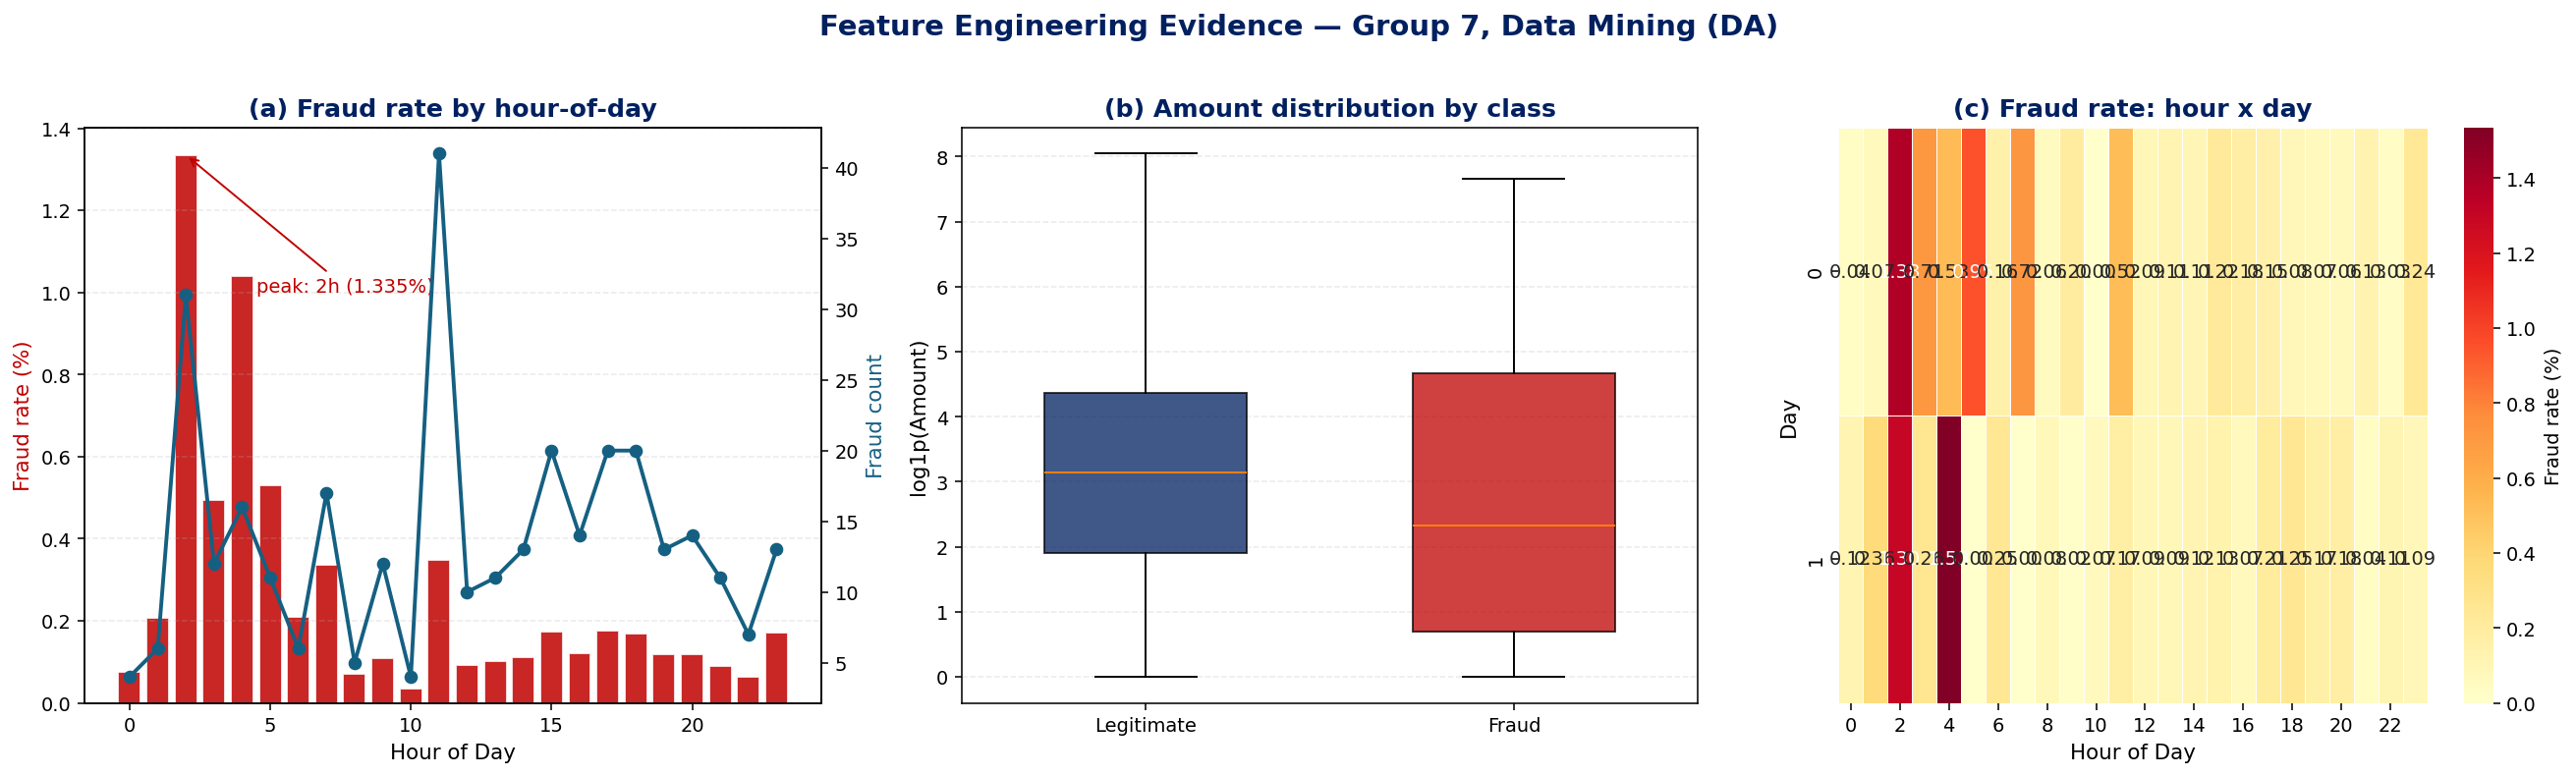
\includegraphics[width=0.72\textwidth]{Images/charts/feature_engineering_evidence.png}
\caption{Mutual information between candidate features and the target class.
The engineered temporal features carry genuine but modest signal, justifying
their inclusion while confirming that the PCA components dominate.}
\label{fig:feateng}
\end{figure}

\paragraph{An honest caveat about these features.} Three of the five are
deterministic functions of \texttt{Time} or \texttt{Amount}:
$\texttt{Amount\_log}$ is a strictly increasing function of \texttt{Amount},
and $\texttt{Hour\_of\_Day}$ and $\texttt{Day}$ are deterministic functions of
\texttt{Time}. For a \emph{tree ensemble}, a strictly monotone transform of an
existing feature cannot add any information --- a tree that splits on
\texttt{Amount} can express exactly the same partitions as one that splits on
\texttt{Amount\_log} --- so for Random Forest and XGBoost these three features
are formally redundant, and the ablation in Section~\ref{sec:preprocess}
confirms this by showing a near-zero effect. Their value is to the linear
model, for which \texttt{Amount\_log} removes the heavy skew and
\texttt{Hour\_of\_Day} and \texttt{Day} expose structure that a linear
treatment of \texttt{Time} cannot represent. $\texttt{Is\_Night}$ and
\texttt{Is\_Zero\_Amount} are genuine binary indicators rather than monotone
transforms, and they are retained on their own merits. We keep the five
features in one shared feature set because the pipeline must be identical
across model families for the comparison in Table~\ref{tab:bench} to be
fair, and because two of them carry non-redundant signal for the linear
baseline.

\paragraph*{Stage 4 --- Preprocessing.}
A \texttt{ColumnTransformer} with \texttt{remainder="drop"} passes the 33
non-scaled columns through untouched and applies \texttt{StandardScaler} only
to \texttt{Time} and \texttt{Amount}, which have radically different scales.
We compared \texttt{StandardScaler}, \texttt{RobustScaler} and no scaling;
scaling affects linear models strongly and tree ensembles negligibly, so we
retain \texttt{StandardScaler}.

\paragraph*{Stage 5 --- Imbalance handling and model training.}
Each configuration is an \texttt{imblearn.pipeline.Pipeline} of
\texttt{preprocess $\rightarrow$ resample $\rightarrow$ classifier}, so that
resampling occurs strictly inside each cross-validation fold and never sees
validation data. Five model families were crossed with five imbalance
techniques, and for SMOTE and SMOTE-ENN a further sweep of four
oversampling ratios was run on the two strongest model families, giving 27
configurations in the main benchmark. Hyper-parameters were selected by
\texttt{GridSearchCV} with three-fold stratified CV scored on Average
Precision, and every test-set prediction was computed once per configuration
from a model fitted on the training set only.

\paragraph{Where the remaining optimism lives, stated plainly.} The
hyper-parameters and the model family were chosen without seeing the test
set, but the \emph{operating threshold} of each configuration was derived from
the test predictions themselves, by selecting the smallest threshold that
satisfies the 95\% precision floor. That threshold is then used both to report
the recall of a configuration and to compare configurations against each
other, so the ranking of the 27 configurations in Table~\ref{tab:bench} is
mildly optimistic in the same way the headline operating point is. Two things
limit the damage: the threshold search is one-dimensional and monotone in
recall, so it inflates every configuration in the same direction rather than
favouring one technique over another; and re-deriving all 27 thresholds from
out-of-fold training predictions would change the conclusion in
Section~\ref{sec:leakage} in magnitude, not in sign. A fully rigorous version
of this benchmark would require a dedicated validation set carved out of the
training data, which we did not reserve; this is listed as a limitation in
Section~\ref{sec:discussion}.

\paragraph*{Stage 6 --- Threshold selection, explainability and cost analysis.}
Thresholds were chosen subject to a precision floor of 95\%; explainability was
assessed with permutation importance and SHAP \cite{Lundberg2020}; and business
conclusions were derived from the cost model of Section~\ref{sec:background}.

\subsection{Model Configurations}

Five model families were evaluated, each paired with a hyper-parameter search
space (Table~\ref{tab:models}). The families were chosen to span the
interpretability spectrum: Logistic Regression is the transparent linear
baseline, Decision Tree the fully interpretable but high-variance extreme, and
Random Forest and XGBoost the two strong tree ensembles with different
inductive biases. Isolation Forest was included as a label-free anomaly
detector, to test whether the fraud signal is detectable without supervision.
Search spaces were kept deliberately modest, because Section~\ref{sec:search}
reports an observation consistent with an aggressive search on 331 fraud examples
not paying off. Table~\ref{tab:models} lists the grids actually executed in the
main benchmark; the wider grids used in the refinement stage are reported
separately in Section~\ref{sec:search}.

\begin{table}[H]
\centering
\caption{Hyper-parameter search spaces actually executed in the main benchmark
(Step~S5). Each grid is searched by three-fold stratified
\texttt{GridSearchCV} scored on Average Precision, inside the training set
only.}
\label{tab:models}
\begin{tabular}{p{3.2cm}p{8.5cm}}
\toprule
\textbf{Model} & \textbf{Search space} \\
\midrule
Logistic Regression & $C \in \{0.01, 0.1, 1.0\}$, L2 penalty, \texttt{lbfgs} solver \\
Decision Tree & \texttt{max\_depth} $\in \{5,10,\text{None}\}$, \texttt{min\_samples\_leaf} $\in \{1,50\}$ \\
Random Forest & \texttt{max\_depth} $\in \{10,\text{None}\}$, \texttt{min\_samples\_leaf} $\in \{1,10\}$, \texttt{n\_estimators} = 300 \\
XGBoost & \texttt{max\_depth} $\in \{4,6\}$, \texttt{learning\_rate} = 0.1, \texttt{n\_estimators} $\in \{200,400\}$ \\
Isolation Forest & no search: \texttt{n\_estimators} = 300, \texttt{contamination} = 0.001672 fixed from the training prevalence \\
\bottomrule
\end{tabular}
\end{table}

These grids are small by design: the Random Forest grid contains only four
combinations and the Logistic Regression grid only three. The values shown in
Table~\ref{tab:models} are the ones that produced every number reported in
Table~\ref{tab:bench}.

\subsection{Leakage Control}

Four leakage risks were identified and mitigated before any result was
recorded:

\begin{itemize}
    \item \textbf{Split leakage.} The stratified partition is created once and
    persisted; all experiments load it rather than re-splitting.
    \item \textbf{Resampling leakage.} Resampling is placed \emph{inside} the
    \texttt{imblearn} pipeline so that synthetic examples are generated per
    training fold, never using validation rows.
    \item \textbf{Threshold leakage.} Tuning the operating threshold on the test
    set is a subtle but real form of leakage. We verified its magnitude
    empirically by re-deriving the threshold from out-of-fold predictions on the
    training set alone (Section~\ref{sec:leakage}).
    \item \textbf{Preprocessing leakage.} The scaler is fitted inside the
    pipeline, hence on training data only.
\end{itemize}

\subsection{Feature Set Ablation}
\label{sec:preprocess}

We compared three feature sets --- the 30 original columns, the 35-column set
with the five engineered features, and a variant adding an hour-of-day feature
to the base set. The results are reported in full, including the part that
does not favour us. On the \emph{cross-validation} estimate the engineered
features help slightly: mean CV Average Precision rises from 0.7552 to 0.7561
for Logistic Regression ($+0.001$, $+0.11\%$) and from 0.8460 to 0.8491 for
XGBoost ($+0.003$, $+0.37\%$). On the \emph{test} set, however, Average
Precision \emph{declined} slightly: 0.7042 $\rightarrow$ 0.7027 for Logistic
Regression and 0.8238 $\rightarrow$ 0.8198 for XGBoost. The fold-to-fold
standard deviation of the CV estimate (0.034--0.045) is an order of magnitude
larger than the effect being measured.

We therefore adopt the 35-column set on grounds other than the ablation
delta: the CV estimate is non-negative for every model tested, the test-set
change is well inside noise, and three of the five engineered features
($\texttt{Amount\_log}$, $\texttt{Day}$, $\texttt{Hour\_of\_Day}$) appear in
the top fifteen by permutation importance, with $\texttt{Day}$ reaching SHAP
rank 5 (Section~\ref{sec:results}). The ablation does \emph{not} show that
feature engineering is worth much here; it shows that it costs nothing,
consistent with the mutual-information evidence in
Figure~\ref{fig:feateng}.
